\chapter{Material de apoyo: uso de agentes de IA para documentación, desarrollo y revisión técnica del proyecto}
\label{annex:ia_collaboration}

\section{Nota de alcance y propósito}
Este capítulo no describe un módulo funcional o componente obligatorio del sistema ANE. Se presenta exclusivamente como \textbf{material de apoyo metodológico} que documenta las técnicas de asistencia técnica utilizadas por el equipo de trabajo. El objetivo es proporcionar una guía sobre cómo el uso responsable de Inteligencia Artificial (IA) ha apoyado la documentación, revisión de código y organización de la información durante el ciclo de vida del proyecto.

\section{Contexto y diferenciación funcional}
Es fundamental diferenciar entre el uso de la IA como herramienta de apoyo al desarrollo y su posible rol como componente funcional del sistema.
\begin{itemize}
    \item \textbf{IA como herramienta de apoyo}: Metodología aplicada para mejorar la productividad, coherencia documental y calidad del código mediante revisión asistida.
    \item \textbf{IA como componente del sistema}: Funcionalidades de análisis inteligente de señales o gestión autónoma que se plantean como propuestas futuras y no forman parte de la arquitectura operativa actual de ANE.
\end{itemize}

\section{Metodología de trabajo: Ecosistema de Agentes}
El equipo emplea herramientas de IA aprobadas institucionalmente para asistir en tareas técnicas. Aunque el enfoque es agnóstico al modelo, se documentan a continuación los pasos de habilitación para las herramientas utilizadas como referencia durante el proyecto.

\subsection{Habilitación del Entorno (Ejemplos CLI)}
Para permitir una interacción directa desde la terminal y facilitar la automatización, se utilizaron los siguientes agentes:

\begin{itemize}
    \item \textbf{GitHub Copilot CLI}: Utilizado para asistencia en codificación y gestión de repositorios.
    \begin{itemize}
        \item Instalación: \texttt{npm install -g @github/copilot}
        \item Autenticación: \texttt{copilot /login}
    \end{itemize}
    \item \textbf{Gemini CLI}: Utilizado para tareas multimodales, análisis de arquitectura y gestión de habilidades.
    \begin{itemize}
        \item Instalación: \texttt{npm install -g @google/gemini-cli}
        \item Inicio: \texttt{gemini}
    \end{itemize}
\end{itemize}

\subsection{Arquitectura Multi-Agente Asistida}
La arquitectura multi-agente se define aquí como una \textbf{metodología de trabajo asistido}, no como una implementación automática dentro del sistema. Se sugieren los siguientes roles para la colaboración:

\begin{itemize}
    \item \textbf{Agente Documental}: Apoyo en redacción técnica, generación de tablas y coherencia de estilo.
    \item \textbf{Agente de Código}: Revisión de scripts, detección de errores lógicos y sugerencias de optimización.
    \item \textbf{Agente de Pruebas}: Generación de casos de prueba y protocolos de validación.
    \item \textbf{Agente de Arquitectura}: Análisis de dependencias y revisión de diagramas de diseño.
    \item \textbf{Agente de Señales/RF}: Apoyo en el análisis de logs y procesamiento teórico de espectro.
    \item \textbf{Agente de Revisión}: Validación cruzada de respuestas para minimizar alucinaciones.
\end{itemize}

\begin{figure}[H]
    \centering
    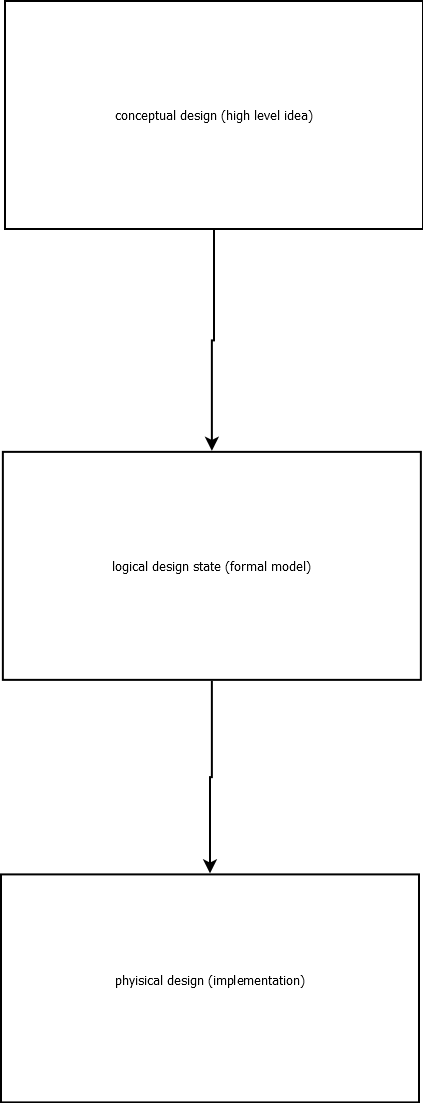
\includegraphics[width=0.4\textwidth]{section/img/annexes/ai_structure.png}
    \caption{Diseño conceptual del sistema multi-agente: Relación metodológica entre roles de asistencia. Fuente: Elaboración propia.}
    \label{fig:ai_conceptual_structure}
\end{figure}

\section{Gobernanza y Uso Responsable de IA}
El uso de herramientas de IA en el proyecto ANE está sujeto a las siguientes restricciones de seguridad y ética:
\begin{itemize}
    \item \textbf{Revisión Humana Obligatoria}: Ningún resultado generado por IA se considera definitivo sin la validación técnica de un responsable humano.
    \item \textbf{Confidencialidad}: Está estrictamente prohibido cargar información sensible, credenciales, llaves de API o datos institucionales restringidos en herramientas externas.
    \item \textbf{No Normatividad}: La IA no es una fuente normativa; las decisiones técnicas se basan en estándares de ingeniería y requerimientos del proyecto.
    \item \textbf{Validación de Código}: No se acepta código sugerido sin pruebas unitarias y validación en el entorno de desarrollo.
\end{itemize}

\section{Trazabilidad Metodológica}
A continuación, se presenta la trazabilidad del uso de IA frente a las actividades de apoyo del proyecto.

\begin{table}[H]
\centering
\caption{Trazabilidad de actividades de apoyo con IA.}
\label{tab:ai_traceability}
\begin{tabularx}{\textwidth}{@{}l X l@{}}
\toprule
Actividad de Apoyo & Aplicación en el Proyecto & Estado \\
\midrule
Documentación Técnica & Generación de estructuras y tablas iniciales. & Aplicado \\
Revisión de Código & Análisis de scripts de adquisición edge. & Parcial \\
Generación de Pruebas & Creación de protocolos de validación HW. & Sugerido \\
Análisis de Errores & Interpretación de logs de comunicación cloud. & Aplicado \\
Organización de Info. & Clasificación de requisitos y dependencias. & Recomendado \\
\bottomrule
\end{tabularx}
\end{table}

\section{Flujo de Trabajo Colaborativo (Paso a Paso)}
Para asegurar la calidad y trazabilidad, se sigue el siguiente flujo:
\begin{enumerate}
    \item \textbf{Definir Tarea}: Clarificar el objetivo técnico y las restricciones.
    \item \textbf{Preparar Contexto}: Seleccionar archivos, logs o requisitos relevantes.
    \item \textbf{Consultar IA}: Utilizar prompts estructurados (ROLE-OBJECTIVE-CONTEXT).
    \item \textbf{Revisar Respuesta}: Identificar posibles errores o inconsistencias.
    \item \textbf{Validar Técnicamente}: Probar el código o verificar los datos en el sistema real.
    \item \textbf{Integrar y Documentar}: Subir al repositorio (GitHub) indicando la asistencia recibida y quién validó.
\end{enumerate}

\section{Trazabilidad de Prompts y Relación con GitHub}
Cada interacción significativa con la IA debe ser trazable. Se recomienda asociar los prompts importantes a:
\begin{itemize}
    \item \textbf{GitHub Issues}: Documentar el prompt usado para resolver un bug específico.
    \item \textbf{Commits/PRs}: Indicar en el mensaje del commit si se utilizó asistencia de IA y quién realizó la revisión final.
    \item \textbf{Archivo de Evidencias}: Registro del prompt, respuesta y decisión tomada.
\end{itemize}

\section{Problemas, Limitaciones y Ajustes}
La IA presenta limitaciones inherentes que deben ser gestionadas mediante supervisión constante.

\begin{longtable}{p{2.6cm} p{3.2cm} p{3cm} p{3cm} p{2.8cm}}
\caption{Gestión de problemas y limitaciones de la IA.}\\
\toprule
\textbf{Problema/Riesgo} & \textbf{Manifestación} & \textbf{Causa} & \textbf{Ajuste/Acción} & \textbf{Resultado} \\
\midrule
\endfirsthead
\toprule
\textbf{Problema/Riesgo} & \textbf{Manifestación} & \textbf{Causa} & \textbf{Ajuste/Acción} & \textbf{Resultado} \\
\midrule
\endhead
Alucinaciones & Librerías inexistentes o comandos falsos. & Falta de datos en el modelo. & Validación cruzada y búsqueda en docs oficiales. & Eliminación de errores técnicos. \\
\midrule
Exposición de Datos & Riesgo de subir credenciales. & Descuido en la preparación de contexto. & Uso de \texttt{.gitignore} y limpieza de prompts. & Integridad de secretos mantenida. \\
\midrule
Dependencia & Pérdida de criterio técnico propio. & Uso excesivo sin razonamiento. & Rotación de tareas y revisión por pares. & Mantenimiento del conocimiento. \\
\bottomrule
\end{longtable}

\section{Métricas de Utilidad y Evidencias}
Para evaluar la efectividad de esta metodología, se consideran las siguientes métricas simples:
\begin{itemize}
    \item \textbf{Tareas Apoyadas}: Número de capítulos o módulos revisados con asistencia.
    \item \textbf{Propuestas Aceptadas/Descartadas}: Porcentaje de sugerencias de IA integradas tras revisión.
    \item \textbf{Tiempo Ahorrado}: Estimación del impacto en la velocidad de documentación y depuración.
\end{itemize}

\begin{figure}[H]
    \centering
    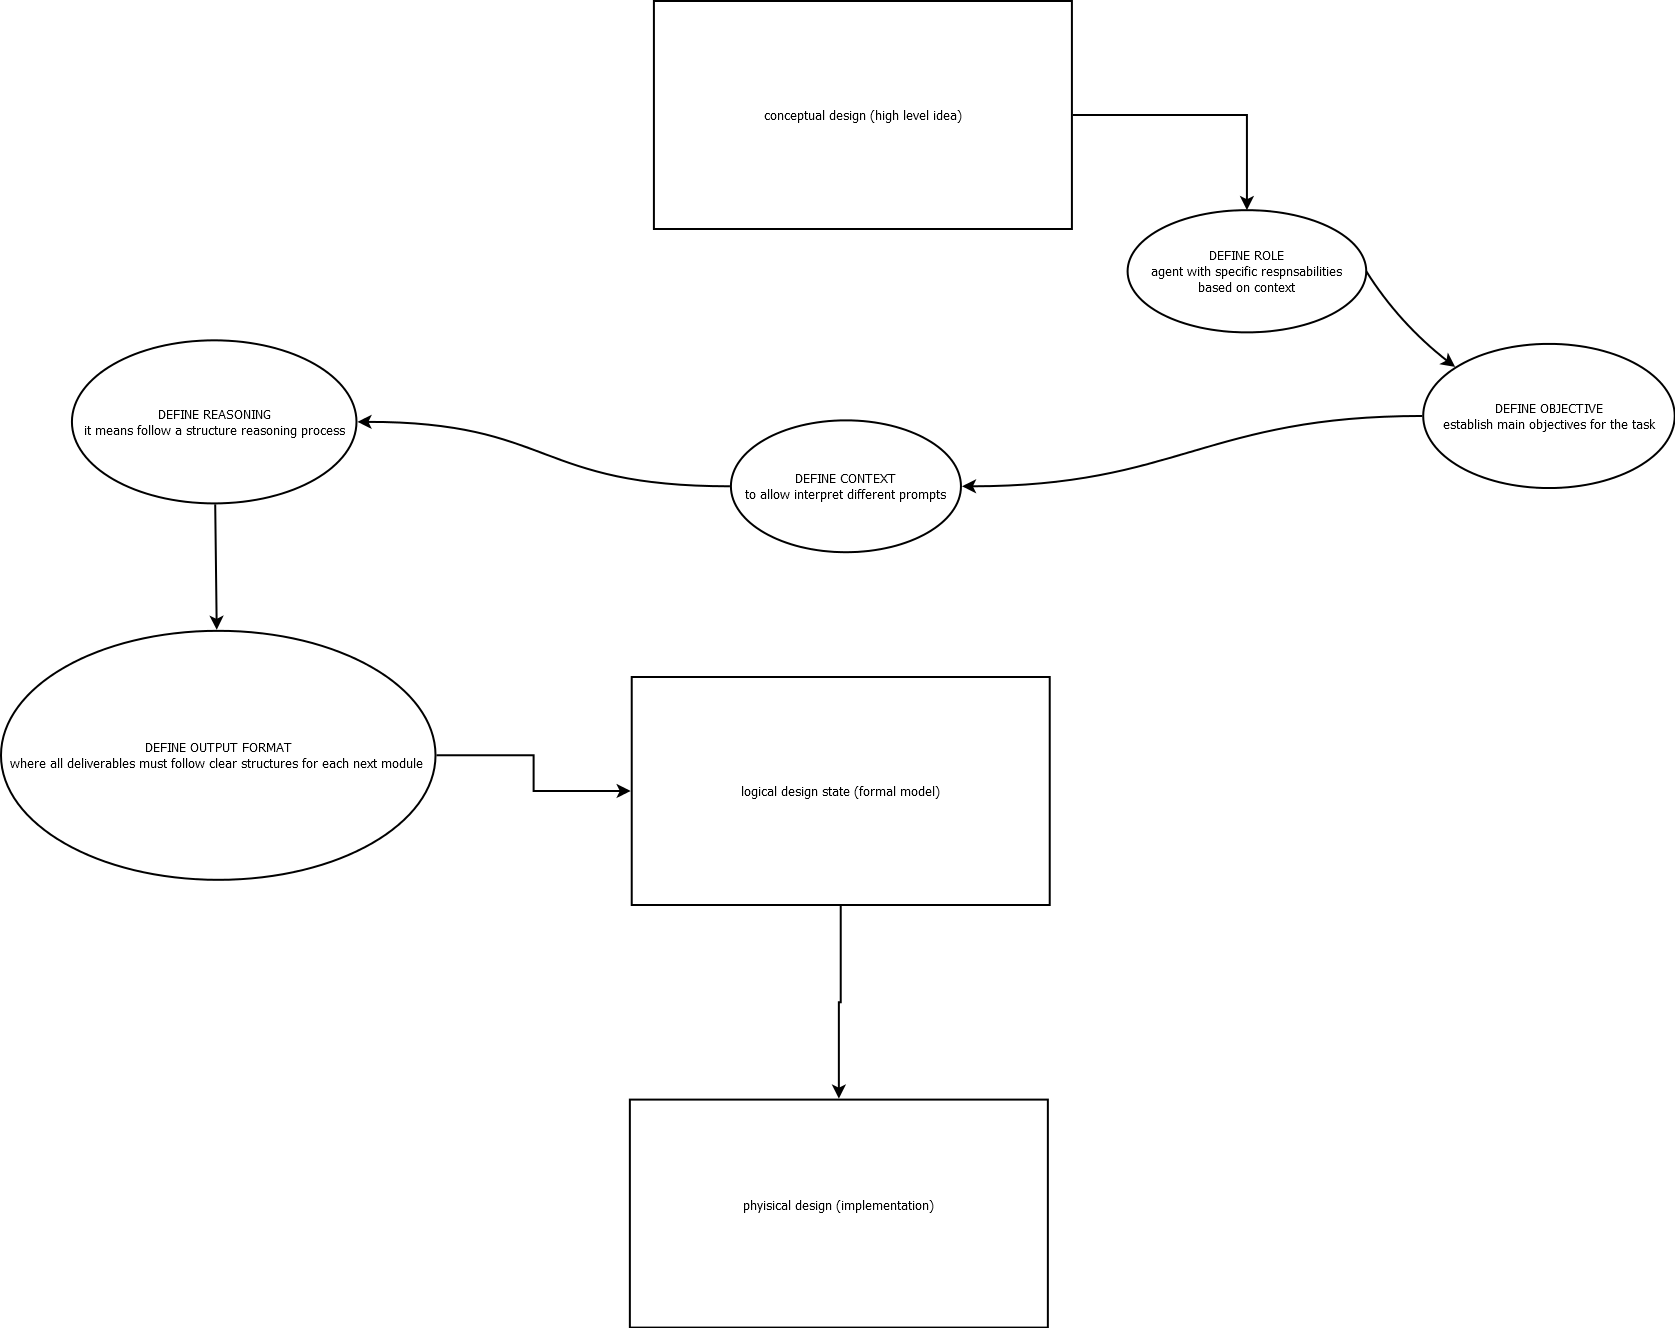
\includegraphics[width=0.8\textwidth]{section/img/annexes/ai_roles.png}
    \caption{Flujo de trabajo y validación humana en la integración de resultados. Fuente: Elaboración propia.}
    \label{fig:ai_roles_workflow}
\end{figure}

\section{Conclusión del capítulo}
La Inteligencia Artificial se propone y utiliza como un multiplicador de productividad para el equipo técnico. Sin embargo, se enfatiza que la responsabilidad final de todas las decisiones, la seguridad del código y la veracidad de la documentación recae exclusivamente en los ingenieros responsables del proyecto. La validación humana es el pilar central que garantiza la integridad del sistema ANE.
